%%%%%%%%%%%%%%%%%%%%%%%%%%%%%%%%%%%%%%%%%%%%%%%%%%
%% Global Statistical Pocketbook 2015
%%%%%%%%%%%%%%%%%%%%%%%%%%%%%%%%%%%%%%%%%%%%%%%%%%

%% Global Pocket Yearbook class
% \documentclass[print, Draft]{faofactbook}
%\documentclass[print]{faofactbook}
%\documentclass[web, Draft]{faofactbook}
\documentclass[twoside,web]{faofactbook}

%% Other packages to be loaded
\usepackage{lipsum,textcomp}
\usepackage[T1]{fontenc}
\usepackage[utf8x]{inputenc}
\usepackage{tabularx}
\usepackage{fixltx2e}
\usepackage{bpchem}
\usepackage{arydshln}
\usepackage{booktabs}
%\usepackage[document]{ragged2e}




\usepackage{array}
\newcolumntype{L}[1]{>{\raggedright\let\newline\\\arraybackslash\hspace{0pt}}m{#1}}
\newcolumntype{C}[1]{>{\centering\let\newline\\\arraybackslash\hspace{0pt}}m{#1}}
\newcolumntype{R}[1]{>{\raggedleft\let\newline\\\arraybackslash\hspace{0pt}}m{#1}}

\PrerenderUnicode {ô}
\makeindex

%% Define the colors
\definecolor{part1}{cmyk}{0.90,0.40,0.24,0.32}
\definecolor{part2}{cmyk}{0,0.54,0.96,0.10}
\definecolor{part3}{cmyk}{0.18,0.90,0.75,0.31}
\definecolor{part4}{cmyk}{0.73,0.10,0.97,0.29}
\definecolor{part5}{cmyk}{0,0,0,0.5}
\definecolor{part6}{cmyk}{0,0,0,0.5}

%% Set the strip width
\faoset{stripwidth=7.2mm}

%% Trying to control the TOC
% \usepackage{tocloft}
% \renewcommand\cftchapfont{\normalsize\bfseries}
% \renewcommand\cftsecfont{\normalsize}

%\usepackage{titlesec}
% \titleformat*{\section}{\Large\bfseries}


% First page background graphics
\usepackage{eso-pic}
\newcommand\taustaeka{%
\put(0,0){%
\parbox[b][\paperheight]{\paperwidth}{%
\vfill
\centering
\includegraphics[width=\paperwidth,height=\paperheight,%
keepaspectratio]{front_cover.pdf}%
\vfill
}}}


\newcommand\taustatoka{%
\put(0,0){%
\parbox[b][\paperheight]{\paperwidth}{%
\vfill
\centering
\includegraphics[width=\paperwidth,height=\paperheight,%
%keepaspectratio]{./cover/front_cover.pdf}%
keepaspectratio]{front_cover_RAP.pdf}%
\vfill
}}}

\usepackage{xcolor}

%% Tango color scheme
\definecolor{Part1}{HTML}{1d5979}
\definecolor{Part2}{HTML}{e07317}
\definecolor{Part3}{HTML}{96212d}
\definecolor{Part4}{HTML}{35802d}

\begin{document}
% \SweaveOpts{concordance=TRUE}
% \SweaveOpts{concordance=TRUE}
\faoset{bgcolor=white}\selectcolor
\twocolumn


%% Cover (just in the web version)
\ifprint\addtocounter{page}{1}\else
% \begin{picture}(0,0)
% \put(-28,-502){\includegraphics[width=\paperwidth,height=\paperheight]{./cover/front_cover_2015.png}}
% \end{picture}
% \renewcommand{\arraystretch}{1.1}
\setlength{\tabcolsep}{4pt}
\normalsize
\CountryData{ World }
      \rowcolors{1}{FAOblue!10}{white}
      \begin{tabular}{L{3.9cm} R{1cm} R{1cm} R{1cm}}
      \toprule
      \multicolumn{1}{c}{} & \multicolumn{1}{c}{ 1992 } & \multicolumn{1}{c}{ 2002 } & \multicolumn{1}{c}{ 2014 } \\
      \midrule
	\multicolumn{4}{l}{\textcolor{FAOblue}{\textbf{\large{Setting}}}} \\ 
	 ~ Total population (mln) & 5\,494.8 ~ \ \ & 6\,280.8 ~ \ \ & 7\,243.7 ~ \ \ \\ 
	 ~ Rural population (mln) & 3\,092.9 ~ \ \ & 3\,284.5 ~ \ \ & 3\,362.5 ~ \ \ \\ 
	 ~ GDP per capita, PPP (const. 2011 I\$) & 8\,724.1 ~ \ \ & 10\,443.5 ~ \ \ & \textit{13\,972.5} ~ \ \ \\ 
	 ~ Mortality rate, under-5 (per 1 000 live births) &  ~ \ \ &  ~ \ \ &  ~ \ \ \\ 
	 ~ Life expectancy at birth (years) & 66.2 ~ \ \ & 68.3 ~ \ \ & \textit{70.8} ~ \ \ \\ 
	 ~ Improved water source (\%  pop.) & 77.1 ~ \ \ & 83.8 ~ \ \ & \textit{89.4} ~ \ \ \\ 
	 ~ Improved sanitation facilities (\% of pop.) & 48.6 ~ \ \ & 57.3 ~ \ \ & \textit{63.7} ~ \ \ \\ 
	 ~ Open defecation (\%) &  ~ \ \ &  ~ \ \ &  ~ \ \ \\ 
	 ~ Cause of death (\%) &  ~ \ \ &  ~ \ \ &  ~ \ \ \\ 
	\multicolumn{4}{l}{\textcolor{FAOblue}{\textbf{\large{Anthropometry}}}} \\ 
	 ~ Low-birthweight babies (\% of births) &  ~ \ \ &  ~ \ \ &  ~ \ \ \\ 
	 ~ Wasting, children under-5 (M/F, \%) &  ~ \ \ &  ~ \ \ &  ~ \ \ \\ 
	 ~ Severe wasting, children under-5 (M/F, \%) &  ~ \ \ &  ~ \ \ &  ~ \ \ \\ 
	 ~ Stunting, children under-5 (M/F, \%) &  ~ \ \ &  ~ \ \ &  ~ \ \ \\ 
	 ~ Underweight, children under-5 (M/F, \%) &  ~ \ \ &  ~ \ \ &  ~ \ \ \\ 
	 ~ Underweight, adults (\%) &  ~ \ \ &  ~ \ \ &  ~ \ \ \\ 
	 ~ Overweight, children (M/F, \%) &  ~ \ \ &  ~ \ \ &  ~ \ \ \\ 
	 ~ Overweight and obesity, adults (M/F, \%) &  ~ \ \ &  ~ \ \ &  ~ \ \ \\ 
	 ~ Prevalence of food over-acquisition (\%)* & 23.1 ~ \ \ & 25.0 ~ \ \ & 29.6 ~ \ \ \\ 
	\multicolumn{4}{l}{\textcolor{FAOblue}{\textbf{\large{Nutritional deficiencies}}}} \\ 
	 ~ Anemia, women (pregnant/non-pregnant, \%) &  ~ \ \ &  ~ \ \ &  ~ \ \ \\ 
	 ~ Anemia, children under-5 (\%) &  ~ \ \ &  ~ \ \ &  ~ \ \ \\ 
	 ~ Vitamin A deficiency, total pop. (\%) &  ~ \ \ &  ~ \ \ &  ~ \ \ \\ 
	 ~ Iodine deficiency, children (\%) &  ~ \ \ &  ~ \ \ &  ~ \ \ \\ 
	 ~ Prevalence of undernourishment (\%)* & 18.7 ~ \ \ & 14.9 ~ \ \ & 11.3 ~ \ \ \\ 
	 ~ Number of people undernourished (mln)* & 1\,014.5 ~ \ \ & 929.9 ~ \ \ & 805.3 ~ \ \ \\ 
	 ~ Depth of food decifit (kcal/cap/day)* & 139 ~ \ \ & 111 ~ \ \ & 84 ~ \ \ \\ 
	\multicolumn{4}{l}{\textcolor{FAOblue}{\textbf{\large{Supplementation}}}} \\ 
	 ~ Vitamin A suppl., children 6-59 mths. (\%) &  ~ \ \ &  ~ \ \ &  ~ \ \ \\ 
	 ~ Iodized salt consumption (\% of households) &  ~ \ \ &  ~ \ \ &  ~ \ \ \\ 
	\multicolumn{4}{l}{\textcolor{FAOblue}{\textbf{\large{Diet}}}} \\ 
	 ~ Exclusive breastfeeding, children $<$ 6 mths. (\%) &  ~ \ \ &  ~ \ \ &  ~ \ \ \\ 
	 ~ Min. dietary diversity, inf. and young child. (\%) &  ~ \ \ &  ~ \ \ &  ~ \ \ \\ 
	 ~ Min. meal frequency, inf. and young child. (\%) &  ~ \ \ &  ~ \ \ &  ~ \ \ \\ 
	 ~ Dietary energy supply (kcal/cap/day)* & 2\,595 ~ \ \ & 2\,719 ~ \ \ & 2\,881 ~ \ \ \\ 
	 ~ Average dietary energy supply adequacy (\%)* & 113 ~ \ \ & 116 ~ \ \ & 122 ~ \ \ \\ 
	 ~ Average protein supply (g/cap/day)* & 69 ~ \ \ & 75 ~ \ \ & \textit{79} ~ \ \ \\ 
	 ~ Average supply of animal protein (g/cap/day)* & 24 ~ \ \ & 28 ~ \ \ & \textit{31} ~ \ \ \\ 
	 ~ Average fat supply (g/cap/day)* & 66 ~ \ \ & 73 ~ \ \ & \textit{81} ~ \ \ \\ 
	\multicolumn{4}{l}{\textcolor{FAOblue}{\textbf{\large{Share of dietary energy supply}}}} \\ 
	 ~ Cereals - excluding beer (\%)* & 50.6 ~ \ \ & 48.1 ~ \ \ & 34.8 ~ \ \ \\ 
	 ~ Starchy roots (\%)* & 5.0 ~ \ \ & 5.1 ~ \ \ & 2.6 ~ \ \ \\ 
	 ~ Sugar and sweeteners (\%)* & 8.7 ~ \ \ & 8.5 ~ \ \ & 16.8 ~ \ \ \\ 
	 ~ Pulses (\%)* & 2.2 ~ \ \ & 2.1 ~ \ \ & 0.6 ~ \ \ \\ 
	 ~ Treenuts (\%)* & 0.3 ~ \ \ & 0.4 ~ \ \ & 0.0 ~ \ \ \\ 
	 ~ Oilcrops (\%)* & 1.6 ~ \ \ & 1.9 ~ \ \ & 0.0 ~ \ \ \\ 
	 ~ Vegetables (\%)* & 2.0 ~ \ \ & 2.8 ~ \ \ & 1.5 ~ \ \ \\ 
	 ~ Fruits - excluding wine (\%)* & 2.5 ~ \ \ & 2.8 ~ \ \ & 3.0 ~ \ \ \\ 
	 ~ Alcoholic beverages (\%)* & 2.5 ~ \ \ & 2.3 ~ \ \ & 10.1 ~ \ \ \\ 
	 ~ Stimulants (\%)* & 0.2 ~ \ \ & 0.2 ~ \ \ & 1.9 ~ \ \ \\ 
	 ~ Meat and offals (\%)* & 7.0 ~ \ \ & 7.7 ~ \ \ & 16.9 ~ \ \ \\ 
	 ~ Vegetable oils and animal fats (\%)* & 10.8 ~ \ \ & 11.3 ~ \ \ & 8.5 ~ \ \ \\ 
	 ~ Fish, seafood and aquatic products (\%)* & 1.0 ~ \ \ & 1.1 ~ \ \ & 1.7 ~ \ \ \\ 
	 ~ Milk - excluding butter (\%)* & 4.4 ~ \ \ & 4.5 ~ \ \ & 7.3 ~ \ \ \\ 
	 ~ Eggs (\%)* & 1.0 ~ \ \ & 1.2 ~ \ \ & 0.6 ~ \ \ \\ 
       \toprule
      \end{tabular}
      \clearpage
\CountryData{ Africa }
      \rowcolors{1}{FAOblue!10}{white}
      \begin{tabular}{L{3.9cm} R{1cm} R{1cm} R{1cm}}
      \toprule
      \multicolumn{1}{c}{} & \multicolumn{1}{c}{ 1992 } & \multicolumn{1}{c}{ 2002 } & \multicolumn{1}{c}{ 2014 } \\
      \midrule
	\multicolumn{4}{l}{\textcolor{FAOblue}{\textbf{\large{Setting}}}} \\ 
	 ~ Total population (mln) & 664.0 ~ \ \ & 847.9 ~ \ \ & 1\,138.2 ~ \ \ \\ 
	 ~ Rural population (mln) & 445.5 ~ \ \ & 540.5 ~ \ \ & 675.5 ~ \ \ \\ 
	 ~ GDP per capita, PPP (const. 2011 I\$) & 3\,137.4 ~ \ \ & 3\,457.7 ~ \ \ & \textit{4\,622.5} ~ \ \ \\ 
	 ~ Mortality rate, under-5 (per 1 000 live births) &  ~ \ \ &  ~ \ \ &  ~ \ \ \\ 
	 ~ Life expectancy at birth (years) & 53.5 ~ \ \ & 53.8 ~ \ \ & \textit{58.8} ~ \ \ \\ 
	 ~ Improved water source (\%  pop.) & 56.1 ~ \ \ & 62.4 ~ \ \ & \textit{68.7} ~ \ \ \\ 
	 ~ Improved sanitation facilities (\% of pop.) & 34.2 ~ \ \ & 37.2 ~ \ \ & \textit{39.4} ~ \ \ \\ 
	 ~ Open defecation (\%) &  ~ \ \ &  ~ \ \ &  ~ \ \ \\ 
	 ~ Cause of death (\%) &  ~ \ \ &  ~ \ \ &  ~ \ \ \\ 
	\multicolumn{4}{l}{\textcolor{FAOblue}{\textbf{\large{Anthropometry}}}} \\ 
	 ~ Low-birthweight babies (\% of births) &  ~ \ \ &  ~ \ \ &  ~ \ \ \\ 
	 ~ Wasting, children under-5 (M/F, \%) &  ~ \ \ &  ~ \ \ &  ~ \ \ \\ 
	 ~ Severe wasting, children under-5 (M/F, \%) &  ~ \ \ &  ~ \ \ &  ~ \ \ \\ 
	 ~ Stunting, children under-5 (M/F, \%) &  ~ \ \ &  ~ \ \ &  ~ \ \ \\ 
	 ~ Underweight, children under-5 (M/F, \%) &  ~ \ \ &  ~ \ \ &  ~ \ \ \\ 
	 ~ Underweight, adults (\%) &  ~ \ \ &  ~ \ \ &  ~ \ \ \\ 
	 ~ Overweight, children (M/F, \%) &  ~ \ \ &  ~ \ \ &  ~ \ \ \\ 
	 ~ Overweight and obesity, adults (M/F, \%) &  ~ \ \ &  ~ \ \ &  ~ \ \ \\ 
	 ~ Prevalence of food over-acquisition (\%)* & 19.7 ~ \ \ & 21.2 ~ \ \ & 26.6 ~ \ \ \\ 
	\multicolumn{4}{l}{\textcolor{FAOblue}{\textbf{\large{Nutritional deficiencies}}}} \\ 
	 ~ Anemia, women (pregnant/non-pregnant, \%) &  ~ \ \ &  ~ \ \ &  ~ \ \ \\ 
	 ~ Anemia, children under-5 (\%) &  ~ \ \ &  ~ \ \ &  ~ \ \ \\ 
	 ~ Vitamin A deficiency, total pop. (\%) &  ~ \ \ &  ~ \ \ &  ~ \ \ \\ 
	 ~ Iodine deficiency, children (\%) &  ~ \ \ &  ~ \ \ &  ~ \ \ \\ 
	 ~ Prevalence of undernourishment (\%)* & 27.7 ~ \ \ & 25.2 ~ \ \ & 20.5 ~ \ \ \\ 
	 ~ Number of people undernourished (mln)* & 182.1 ~ \ \ & 209.0 ~ \ \ & 226.7 ~ \ \ \\ 
	 ~ Depth of food decifit (kcal/cap/day)* & 205 ~ \ \ & 185 ~ \ \ & 156 ~ \ \ \\ 
	\multicolumn{4}{l}{\textcolor{FAOblue}{\textbf{\large{Supplementation}}}} \\ 
	 ~ Vitamin A suppl., children 6-59 mths. (\%) &  ~ \ \ &  ~ \ \ &  ~ \ \ \\ 
	 ~ Iodized salt consumption (\% of households) &  ~ \ \ &  ~ \ \ &  ~ \ \ \\ 
	\multicolumn{4}{l}{\textcolor{FAOblue}{\textbf{\large{Diet}}}} \\ 
	 ~ Exclusive breastfeeding, children $<$ 6 mths. (\%) &  ~ \ \ &  ~ \ \ &  ~ \ \ \\ 
	 ~ Min. dietary diversity, inf. and young child. (\%) &  ~ \ \ &  ~ \ \ &  ~ \ \ \\ 
	 ~ Min. meal frequency, inf. and young child. (\%) &  ~ \ \ &  ~ \ \ &  ~ \ \ \\ 
	 ~ Dietary energy supply (kcal/cap/day)* & 2\,320 ~ \ \ & 2\,414 ~ \ \ & 2\,558 ~ \ \ \\ 
	 ~ Average dietary energy supply adequacy (\%)* & 107 ~ \ \ & 110 ~ \ \ & 116 ~ \ \ \\ 
	 ~ Average protein supply (g/cap/day)* & 59 ~ \ \ & 60 ~ \ \ & \textit{65} ~ \ \ \\ 
	 ~ Average supply of animal protein (g/cap/day)* & 13 ~ \ \ & 12 ~ \ \ & \textit{14} ~ \ \ \\ 
	 ~ Average fat supply (g/cap/day)* & 49 ~ \ \ & 48 ~ \ \ & \textit{53} ~ \ \ \\ 
	\multicolumn{4}{l}{\textcolor{FAOblue}{\textbf{\large{Share of dietary energy supply}}}} \\ 
	 ~ Cereals - excluding beer (\%)* & 52.3 ~ \ \ & 51.3 ~ \ \ & \textit{50.6} ~ \ \ \\ 
	 ~ Starchy roots (\%)* & 11.9 ~ \ \ & 12.9 ~ \ \ & \textit{13.5} ~ \ \ \\ 
	 ~ Sugar and sweeteners (\%)* & 6.2 ~ \ \ & 6.4 ~ \ \ & \textit{6.0} ~ \ \ \\ 
	 ~ Pulses (\%)* & 3.4 ~ \ \ & 3.7 ~ \ \ & \textit{4.0} ~ \ \ \\ 
	 ~ Treenuts (\%)* & 0.3 ~ \ \ & 0.5 ~ \ \ & \textit{0.6} ~ \ \ \\ 
	 ~ Oilcrops (\%)* & 1.6 ~ \ \ & 2.2 ~ \ \ & \textit{2.6} ~ \ \ \\ 
	 ~ Vegetables (\%)* & 1.5 ~ \ \ & 1.7 ~ \ \ & \textit{1.8} ~ \ \ \\ 
	 ~ Fruits - excluding wine (\%)* & 3.7 ~ \ \ & 4.0 ~ \ \ & \textit{4.2} ~ \ \ \\ 
	 ~ Alcoholic beverages (\%)* & 1.9 ~ \ \ & 1.8 ~ \ \ & \textit{1.8} ~ \ \ \\ 
	 ~ Stimulants (\%)* & 0.1 ~ \ \ & 0.1 ~ \ \ & \textit{0.1} ~ \ \ \\ 
	 ~ Meat and offals (\%)* & 3.4 ~ \ \ & 3.4 ~ \ \ & \textit{3.5} ~ \ \ \\ 
	 ~ Vegetable oils and animal fats (\%)* & 9.4 ~ \ \ & 9.2 ~ \ \ & \textit{9.3} ~ \ \ \\ 
	 ~ Fish, seafood and aquatic products (\%)* & 0.6 ~ \ \ & 0.6 ~ \ \ & \textit{0.8} ~ \ \ \\ 
	 ~ Milk - excluding butter (\%)* & 2.7 ~ \ \ & 2.9 ~ \ \ & \textit{2.7} ~ \ \ \\ 
	 ~ Eggs (\%)* & 0.3 ~ \ \ & 0.3 ~ \ \ & \textit{0.4} ~ \ \ \\ 
       \toprule
      \end{tabular}
      \clearpage
\CountryData{ Asia }
      \rowcolors{1}{FAOblue!10}{white}
      \begin{tabular}{L{3.9cm} R{1cm} R{1cm} R{1cm}}
      \toprule
      \multicolumn{1}{c}{} & \multicolumn{1}{c}{ 1992 } & \multicolumn{1}{c}{ 2002 } & \multicolumn{1}{c}{ 2014 } \\
      \midrule
	\multicolumn{4}{l}{\textcolor{FAOblue}{\textbf{\large{Setting}}}} \\ 
	 ~ Total population (mln) & 3\,197.6 ~ \ \ & 3\,674.5 ~ \ \ & 4\,206.3 ~ \ \ \\ 
	 ~ Rural population (mln) & 2\,192.8 ~ \ \ & 2\,306.0 ~ \ \ & 2\,283.5 ~ \ \ \\ 
	 ~ GDP per capita, PPP (const. 2011 I\$) & 3\,191.9 ~ \ \ & 4\,932.1 ~ \ \ & \textit{9\,418.0} ~ \ \ \\ 
	 ~ Mortality rate, under-5 (per 1 000 live births) &  ~ \ \ &  ~ \ \ &  ~ \ \ \\ 
	 ~ Life expectancy at birth (years) & 65.3 ~ \ \ & 68.4 ~ \ \ & \textit{71.0} ~ \ \ \\ 
	 ~ Improved water source (\%  pop.) & 73.0 ~ \ \ & 83.0 ~ \ \ & \textit{91.2} ~ \ \ \\ 
	 ~ Improved sanitation facilities (\% of pop.) & 34.1 ~ \ \ & 47.5 ~ \ \ & \textit{58.6} ~ \ \ \\ 
	 ~ Open defecation (\%) &  ~ \ \ &  ~ \ \ &  ~ \ \ \\ 
	 ~ Cause of death (\%) &  ~ \ \ &  ~ \ \ &  ~ \ \ \\ 
	\multicolumn{4}{l}{\textcolor{FAOblue}{\textbf{\large{Anthropometry}}}} \\ 
	 ~ Low-birthweight babies (\% of births) &  ~ \ \ &  ~ \ \ &  ~ \ \ \\ 
	 ~ Wasting, children under-5 (M/F, \%) &  ~ \ \ &  ~ \ \ &  ~ \ \ \\ 
	 ~ Severe wasting, children under-5 (M/F, \%) &  ~ \ \ &  ~ \ \ &  ~ \ \ \\ 
	 ~ Stunting, children under-5 (M/F, \%) &  ~ \ \ &  ~ \ \ &  ~ \ \ \\ 
	 ~ Underweight, children under-5 (M/F, \%) &  ~ \ \ &  ~ \ \ &  ~ \ \ \\ 
	 ~ Underweight, adults (\%) &  ~ \ \ &  ~ \ \ &  ~ \ \ \\ 
	 ~ Overweight, children (M/F, \%) &  ~ \ \ &  ~ \ \ &  ~ \ \ \\ 
	 ~ Overweight and obesity, adults (M/F, \%) &  ~ \ \ &  ~ \ \ &  ~ \ \ \\ 
	 ~ Prevalence of food over-acquisition (\%)* & 17.6 ~ \ \ & 20.0 ~ \ \ & 25.3 ~ \ \ \\ 
	\multicolumn{4}{l}{\textcolor{FAOblue}{\textbf{\large{Nutritional deficiencies}}}} \\ 
	 ~ Anemia, women (pregnant/non-pregnant, \%) &  ~ \ \ &  ~ \ \ &  ~ \ \ \\ 
	 ~ Anemia, children under-5 (\%) &  ~ \ \ &  ~ \ \ &  ~ \ \ \\ 
	 ~ Vitamin A deficiency, total pop. (\%) &  ~ \ \ &  ~ \ \ &  ~ \ \ \\ 
	 ~ Iodine deficiency, children (\%) &  ~ \ \ &  ~ \ \ &  ~ \ \ \\ 
	 ~ Prevalence of undernourishment (\%)* & 23.7 ~ \ \ & 17.6 ~ \ \ & 12.7 ~ \ \ \\ 
	 ~ Number of people undernourished (mln)* & 742.6 ~ \ \ & 637.5 ~ \ \ & 525.6 ~ \ \ \\ 
	 ~ Depth of food decifit (kcal/cap/day)* & 177 ~ \ \ & 131 ~ \ \ & 94 ~ \ \ \\ 
	\multicolumn{4}{l}{\textcolor{FAOblue}{\textbf{\large{Supplementation}}}} \\ 
	 ~ Vitamin A suppl., children 6-59 mths. (\%) &  ~ \ \ &  ~ \ \ &  ~ \ \ \\ 
	 ~ Iodized salt consumption (\% of households) &  ~ \ \ &  ~ \ \ &  ~ \ \ \\ 
	\multicolumn{4}{l}{\textcolor{FAOblue}{\textbf{\large{Diet}}}} \\ 
	 ~ Exclusive breastfeeding, children $<$ 6 mths. (\%) &  ~ \ \ &  ~ \ \ &  ~ \ \ \\ 
	 ~ Min. dietary diversity, inf. and young child. (\%) &  ~ \ \ &  ~ \ \ &  ~ \ \ \\ 
	 ~ Min. meal frequency, inf. and young child. (\%) &  ~ \ \ &  ~ \ \ &  ~ \ \ \\ 
	 ~ Dietary energy supply (kcal/cap/day)* & 2\,397 ~ \ \ & 2\,568 ~ \ \ & 2\,788 ~ \ \ \\ 
	 ~ Average dietary energy supply adequacy (\%)* & 107 ~ \ \ & 111 ~ \ \ & 119 ~ \ \ \\ 
	 ~ Average protein supply (g/cap/day)* & 60 ~ \ \ & 68 ~ \ \ & \textit{75} ~ \ \ \\ 
	 ~ Average supply of animal protein (g/cap/day)* & 14 ~ \ \ & 19 ~ \ \ & \textit{25} ~ \ \ \\ 
	 ~ Average fat supply (g/cap/day)* & 49 ~ \ \ & 59 ~ \ \ & \textit{71} ~ \ \ \\ 
	\multicolumn{4}{l}{\textcolor{FAOblue}{\textbf{\large{Share of dietary energy supply}}}} \\ 
	 ~ Cereals - excluding beer (\%)* & 62.7 ~ \ \ & 57.5 ~ \ \ & \textit{52.7} ~ \ \ \\ 
	 ~ Starchy roots (\%)* & 4.1 ~ \ \ & 4.0 ~ \ \ & \textit{3.6} ~ \ \ \\ 
	 ~ Sugar and sweeteners (\%)* & 6.0 ~ \ \ & 6.1 ~ \ \ & \textit{5.9} ~ \ \ \\ 
	 ~ Pulses (\%)* & 2.3 ~ \ \ & 2.0 ~ \ \ & \textit{2.2} ~ \ \ \\ 
	 ~ Treenuts (\%)* & 0.2 ~ \ \ & 0.3 ~ \ \ & \textit{0.5} ~ \ \ \\ 
	 ~ Oilcrops (\%)* & 2.0 ~ \ \ & 2.2 ~ \ \ & \textit{2.2} ~ \ \ \\ 
	 ~ Vegetables (\%)* & 2.2 ~ \ \ & 3.4 ~ \ \ & \textit{4.1} ~ \ \ \\ 
	 ~ Fruits - excluding wine (\%)* & 1.7 ~ \ \ & 2.3 ~ \ \ & \textit{2.9} ~ \ \ \\ 
	 ~ Alcoholic beverages (\%)* & 1.3 ~ \ \ & 1.3 ~ \ \ & \textit{1.6} ~ \ \ \\ 
	 ~ Stimulants (\%)* & 0.0 ~ \ \ & 0.1 ~ \ \ & \textit{0.1} ~ \ \ \\ 
	 ~ Meat and offals (\%)* & 5.3 ~ \ \ & 6.8 ~ \ \ & \textit{7.9} ~ \ \ \\ 
	 ~ Vegetable oils and animal fats (\%)* & 7.7 ~ \ \ & 8.6 ~ \ \ & \textit{9.7} ~ \ \ \\ 
	 ~ Fish, seafood and aquatic products (\%)* & 0.8 ~ \ \ & 1.1 ~ \ \ & \textit{1.3} ~ \ \ \\ 
	 ~ Milk - excluding butter (\%)* & 2.4 ~ \ \ & 2.6 ~ \ \ & \textit{3.3} ~ \ \ \\ 
	 ~ Eggs (\%)* & 0.7 ~ \ \ & 1.2 ~ \ \ & \textit{1.3} ~ \ \ \\ 
       \toprule
      \end{tabular}
      \clearpage
\CountryData{ Latin America and the Caribbean }
      \rowcolors{1}{FAOblue!10}{white}
      \begin{tabular}{L{3.9cm} R{1cm} R{1cm} R{1cm}}
      \toprule
      \multicolumn{1}{c}{} & \multicolumn{1}{c}{ 1992 } & \multicolumn{1}{c}{ 2002 } & \multicolumn{1}{c}{ 2014 } \\
      \midrule
	\multicolumn{4}{l}{\textcolor{FAOblue}{\textbf{\large{Setting}}}} \\ 
	 ~ Total population (mln) & 461.6 ~ \ \ & 541.1 ~ \ \ & 623.3 ~ \ \ \\ 
	 ~ Rural population (mln) & 131.7 ~ \ \ & 128.7 ~ \ \ & 124.9 ~ \ \ \\ 
	 ~ GDP per capita, PPP (const. 2011 I\$) & 9\,930.9 ~ \ \ & 10\,899.1 ~ \ \ & \textit{13\,753.7} ~ \ \ \\ 
	 ~ Mortality rate, under-5 (per 1 000 live births) &  ~ \ \ &  ~ \ \ &  ~ \ \ \\ 
	 ~ Life expectancy at birth (years) & 69.0 ~ \ \ & 72.2 ~ \ \ & \textit{74.6} ~ \ \ \\ 
	 ~ Improved water source (\%  pop.) & 86.1 ~ \ \ & 90.5 ~ \ \ & \textit{94.0} ~ \ \ \\ 
	 ~ Improved sanitation facilities (\% of pop.) & 69.0 ~ \ \ & 76.3 ~ \ \ & \textit{81.7} ~ \ \ \\ 
	 ~ Open defecation (\%) &  ~ \ \ &  ~ \ \ &  ~ \ \ \\ 
	 ~ Cause of death (\%) &  ~ \ \ &  ~ \ \ &  ~ \ \ \\ 
	\multicolumn{4}{l}{\textcolor{FAOblue}{\textbf{\large{Anthropometry}}}} \\ 
	 ~ Low-birthweight babies (\% of births) &  ~ \ \ &  ~ \ \ &  ~ \ \ \\ 
	 ~ Wasting, children under-5 (M/F, \%) &  ~ \ \ &  ~ \ \ &  ~ \ \ \\ 
	 ~ Severe wasting, children under-5 (M/F, \%) &  ~ \ \ &  ~ \ \ &  ~ \ \ \\ 
	 ~ Stunting, children under-5 (M/F, \%) &  ~ \ \ &  ~ \ \ &  ~ \ \ \\ 
	 ~ Underweight, children under-5 (M/F, \%) &  ~ \ \ &  ~ \ \ &  ~ \ \ \\ 
	 ~ Underweight, adults (\%) &  ~ \ \ &  ~ \ \ &  ~ \ \ \\ 
	 ~ Overweight, children (M/F, \%) &  ~ \ \ &  ~ \ \ &  ~ \ \ \\ 
	 ~ Overweight and obesity, adults (M/F, \%) &  ~ \ \ &  ~ \ \ &  ~ \ \ \\ 
	 ~ Prevalence of food over-acquisition (\%)* & 24.5 ~ \ \ & 27.2 ~ \ \ & 32.9 ~ \ \ \\ 
	\multicolumn{4}{l}{\textcolor{FAOblue}{\textbf{\large{Nutritional deficiencies}}}} \\ 
	 ~ Anemia, women (pregnant/non-pregnant, \%) &  ~ \ \ &  ~ \ \ &  ~ \ \ \\ 
	 ~ Anemia, children under-5 (\%) &  ~ \ \ &  ~ \ \ &  ~ \ \ \\ 
	 ~ Vitamin A deficiency, total pop. (\%) &  ~ \ \ &  ~ \ \ &  ~ \ \ \\ 
	 ~ Iodine deficiency, children (\%) &  ~ \ \ &  ~ \ \ &  ~ \ \ \\ 
	 ~ Prevalence of undernourishment (\%)* & 15.3 ~ \ \ & 11.5 ~ \ \ & 6.1 ~ \ \ \\ 
	 ~ Number of people undernourished (mln)* & 68.5 ~ \ \ & 61.0 ~ \ \ & 37.0 ~ \ \ \\ 
	 ~ Depth of food decifit (kcal/cap/day)* & 109 ~ \ \ & 83 ~ \ \ & 44 ~ \ \ \\ 
	\multicolumn{4}{l}{\textcolor{FAOblue}{\textbf{\large{Supplementation}}}} \\ 
	 ~ Vitamin A suppl., children 6-59 mths. (\%) &  ~ \ \ &  ~ \ \ &  ~ \ \ \\ 
	 ~ Iodized salt consumption (\% of households) &  ~ \ \ &  ~ \ \ &  ~ \ \ \\ 
	\multicolumn{4}{l}{\textcolor{FAOblue}{\textbf{\large{Diet}}}} \\ 
	 ~ Exclusive breastfeeding, children $<$ 6 mths. (\%) &  ~ \ \ &  ~ \ \ &  ~ \ \ \\ 
	 ~ Min. dietary diversity, inf. and young child. (\%) &  ~ \ \ &  ~ \ \ &  ~ \ \ \\ 
	 ~ Min. meal frequency, inf. and young child. (\%) &  ~ \ \ &  ~ \ \ &  ~ \ \ \\ 
	 ~ Dietary energy supply (kcal/cap/day)* & 2\,655 ~ \ \ & 2\,792 ~ \ \ & 3\,010 ~ \ \ \\ 
	 ~ Average dietary energy supply adequacy (\%)* & 116 ~ \ \ & 120 ~ \ \ & 127 ~ \ \ \\ 
	 ~ Average protein supply (g/cap/day)* & 68 ~ \ \ & 77 ~ \ \ & \textit{82} ~ \ \ \\ 
	 ~ Average supply of animal protein (g/cap/day)* & 30 ~ \ \ & 37 ~ \ \ & \textit{42} ~ \ \ \\ 
	 ~ Average fat supply (g/cap/day)* & 73 ~ \ \ & 84 ~ \ \ & \textit{93} ~ \ \ \\ 
	\multicolumn{4}{l}{\textcolor{FAOblue}{\textbf{\large{Share of dietary energy supply}}}} \\ 
	 ~ Cereals - excluding beer (\%)* & 38.4 ~ \ \ & 36.7 ~ \ \ & 33.3 ~ \ \ \\ 
	 ~ Starchy roots (\%)* & 4.2 ~ \ \ & 4.1 ~ \ \ & 2.5 ~ \ \ \\ 
	 ~ Sugar and sweeteners (\%)* & 16.1 ~ \ \ & 14.3 ~ \ \ & 16.1 ~ \ \ \\ 
	 ~ Pulses (\%)* & 3.8 ~ \ \ & 3.7 ~ \ \ & 0.6 ~ \ \ \\ 
	 ~ Treenuts (\%)* & 0.1 ~ \ \ & 0.2 ~ \ \ & 0.0 ~ \ \ \\ 
	 ~ Oilcrops (\%)* & 0.8 ~ \ \ & 1.4 ~ \ \ & 0.0 ~ \ \ \\ 
	 ~ Vegetables (\%)* & 1.1 ~ \ \ & 1.3 ~ \ \ & 1.4 ~ \ \ \\ 
	 ~ Fruits - excluding wine (\%)* & 4.3 ~ \ \ & 4.4 ~ \ \ & 2.9 ~ \ \ \\ 
	 ~ Alcoholic beverages (\%)* & 2.6 ~ \ \ & 2.5 ~ \ \ & 9.6 ~ \ \ \\ 
	 ~ Stimulants (\%)* & 0.2 ~ \ \ & 0.3 ~ \ \ & 1.8 ~ \ \ \\ 
	 ~ Meat and offals (\%)* & 8.3 ~ \ \ & 10.2 ~ \ \ & 16.1 ~ \ \ \\ 
	 ~ Vegetable oils and animal fats (\%)* & 12.7 ~ \ \ & 12.7 ~ \ \ & 8.1 ~ \ \ \\ 
	 ~ Fish, seafood and aquatic products (\%)* & 0.5 ~ \ \ & 0.6 ~ \ \ & 1.6 ~ \ \ \\ 
	 ~ Milk - excluding butter (\%)* & 5.5 ~ \ \ & 6.2 ~ \ \ & 7.0 ~ \ \ \\ 
	 ~ Eggs (\%)* & 1.0 ~ \ \ & 1.1 ~ \ \ & 0.5 ~ \ \ \\ 
       \toprule
      \end{tabular}
      \clearpage
\CountryData{ Oceania }
      \rowcolors{1}{FAOblue!10}{white}
      \begin{tabular}{L{3.9cm} R{1cm} R{1cm} R{1cm}}
      \toprule
      \multicolumn{1}{c}{} & \multicolumn{1}{c}{ 1992 } & \multicolumn{1}{c}{ 2002 } & \multicolumn{1}{c}{ 2014 } \\
      \midrule
	\multicolumn{4}{l}{\textcolor{FAOblue}{\textbf{\large{Setting}}}} \\ 
	 ~ Total population (mln) & 6.8 ~ \ \ & 8.4 ~ \ \ & 10.6 ~ \ \ \\ 
	 ~ Rural population (mln) & 5.1 ~ \ \ & 6.5 ~ \ \ & 8.3 ~ \ \ \\ 
	 ~ GDP per capita, PPP (const. 2011 I\$) & 2\,562.3 ~ \ \ & 2\,505.3 ~ \ \ & \textit{3\,038.2} ~ \ \ \\ 
	 ~ Mortality rate, under-5 (per 1 000 live births) &  ~ \ \ &  ~ \ \ &  ~ \ \ \\ 
	 ~ Life expectancy at birth (years) & 59.5 ~ \ \ & 62.5 ~ \ \ & \textit{64.9} ~ \ \ \\ 
	 ~ Improved water source (\%  pop.) & 49.6 ~ \ \ & 53.5 ~ \ \ & \textit{55.5} ~ \ \ \\ 
	 ~ Improved sanitation facilities (\% of pop.) & 35.6 ~ \ \ & 35.4 ~ \ \ & \textit{35.1} ~ \ \ \\ 
	 ~ Open defecation (\%) &  ~ \ \ &  ~ \ \ &  ~ \ \ \\ 
	 ~ Cause of death (\%) &  ~ \ \ &  ~ \ \ &  ~ \ \ \\ 
	\multicolumn{4}{l}{\textcolor{FAOblue}{\textbf{\large{Anthropometry}}}} \\ 
	 ~ Low-birthweight babies (\% of births) &  ~ \ \ &  ~ \ \ &  ~ \ \ \\ 
	 ~ Wasting, children under-5 (M/F, \%) &  ~ \ \ &  ~ \ \ &  ~ \ \ \\ 
	 ~ Severe wasting, children under-5 (M/F, \%) &  ~ \ \ &  ~ \ \ &  ~ \ \ \\ 
	 ~ Stunting, children under-5 (M/F, \%) &  ~ \ \ &  ~ \ \ &  ~ \ \ \\ 
	 ~ Underweight, children under-5 (M/F, \%) &  ~ \ \ &  ~ \ \ &  ~ \ \ \\ 
	 ~ Underweight, adults (\%) &  ~ \ \ &  ~ \ \ &  ~ \ \ \\ 
	 ~ Overweight, children (M/F, \%) &  ~ \ \ &  ~ \ \ &  ~ \ \ \\ 
	 ~ Overweight and obesity, adults (M/F, \%) &  ~ \ \ &  ~ \ \ &  ~ \ \ \\ 
	 ~ Prevalence of food over-acquisition (\%)* & 19.3 ~ \ \ & 18.2 ~ \ \ & 20.6 ~ \ \ \\ 
	\multicolumn{4}{l}{\textcolor{FAOblue}{\textbf{\large{Nutritional deficiencies}}}} \\ 
	 ~ Anemia, women (pregnant/non-pregnant, \%) &  ~ \ \ &  ~ \ \ &  ~ \ \ \\ 
	 ~ Anemia, children under-5 (\%) &  ~ \ \ &  ~ \ \ &  ~ \ \ \\ 
	 ~ Vitamin A deficiency, total pop. (\%) &  ~ \ \ &  ~ \ \ &  ~ \ \ \\ 
	 ~ Iodine deficiency, children (\%) &  ~ \ \ &  ~ \ \ &  ~ \ \ \\ 
	 ~ Prevalence of undernourishment (\%)* & 15.7 ~ \ \ & 16.5 ~ \ \ & 14.0 ~ \ \ \\ 
	 ~ Number of people undernourished (mln)* & 1.0 ~ \ \ & 1.3 ~ \ \ & 1.4 ~ \ \ \\ 
	 ~ Depth of food decifit (kcal/cap/day)* & 101 ~ \ \ & 107 ~ \ \ & 92 ~ \ \ \\ 
	\multicolumn{4}{l}{\textcolor{FAOblue}{\textbf{\large{Supplementation}}}} \\ 
	 ~ Vitamin A suppl., children 6-59 mths. (\%) &  ~ \ \ &  ~ \ \ &  ~ \ \ \\ 
	 ~ Iodized salt consumption (\% of households) &  ~ \ \ &  ~ \ \ &  ~ \ \ \\ 
	\multicolumn{4}{l}{\textcolor{FAOblue}{\textbf{\large{Diet}}}} \\ 
	 ~ Exclusive breastfeeding, children $<$ 6 mths. (\%) &  ~ \ \ &  ~ \ \ &  ~ \ \ \\ 
	 ~ Min. dietary diversity, inf. and young child. (\%) &  ~ \ \ &  ~ \ \ &  ~ \ \ \\ 
	 ~ Min. meal frequency, inf. and young child. (\%) &  ~ \ \ &  ~ \ \ &  ~ \ \ \\ 
	 ~ Dietary energy supply (kcal/cap/day)* & 2\,454 ~ \ \ & 2\,438 ~ \ \ & 2\,539 ~ \ \ \\ 
	 ~ Average dietary energy supply adequacy (\%)* & 113 ~ \ \ & 112 ~ \ \ & 115 ~ \ \ \\ 
	 ~ Average protein supply (g/cap/day)* & 70 ~ \ \ & 69 ~ \ \ & \textit{72} ~ \ \ \\ 
	 ~ Average supply of animal protein (g/cap/day)* & 39 ~ \ \ & 36 ~ \ \ & \textit{38} ~ \ \ \\ 
	 ~ Average fat supply (g/cap/day)* & 65 ~ \ \ & 62 ~ \ \ & \textit{60} ~ \ \ \\ 
	\multicolumn{4}{l}{\textcolor{FAOblue}{\textbf{\large{Share of dietary energy supply}}}} \\ 
	 ~ Cereals - excluding beer (\%)* & 35.9 ~ \ \ & 39.2 ~ \ \ & \textit{36.5} ~ \ \ \\ 
	 ~ Starchy roots (\%)* & 12.4 ~ \ \ & 14.4 ~ \ \ & \textit{14.9} ~ \ \ \\ 
	 ~ Sugar and sweeteners (\%)* & 9.0 ~ \ \ & 8.9 ~ \ \ & \textit{9.5} ~ \ \ \\ 
	 ~ Pulses (\%)* & 1.8 ~ \ \ & 2.1 ~ \ \ & \textit{2.0} ~ \ \ \\ 
	 ~ Treenuts (\%)* & 0.1 ~ \ \ & 0.2 ~ \ \ & \textit{0.2} ~ \ \ \\ 
	 ~ Oilcrops (\%)* & 10.4 ~ \ \ & 10.5 ~ \ \ & \textit{10.7} ~ \ \ \\ 
	 ~ Vegetables (\%)* & 1.0 ~ \ \ & 1.2 ~ \ \ & \textit{1.2} ~ \ \ \\ 
	 ~ Fruits - excluding wine (\%)* & 2.5 ~ \ \ & 2.7 ~ \ \ & \textit{3.0} ~ \ \ \\ 
	 ~ Alcoholic beverages (\%)* & 1.6 ~ \ \ & 1.6 ~ \ \ & \textit{1.7} ~ \ \ \\ 
	 ~ Stimulants (\%)* & 0.4 ~ \ \ & 0.5 ~ \ \ & \textit{0.6} ~ \ \ \\ 
	 ~ Meat and offals (\%)* & 10.8 ~ \ \ & 10.8 ~ \ \ & \textit{10.0} ~ \ \ \\ 
	 ~ Vegetable oils and animal fats (\%)* & 12.3 ~ \ \ & 12.8 ~ \ \ & \textit{12.1} ~ \ \ \\ 
	 ~ Fish, seafood and aquatic products (\%)* & 2.9 ~ \ \ & 3.0 ~ \ \ & \textit{3.1} ~ \ \ \\ 
	 ~ Milk - excluding butter (\%)* & 3.6 ~ \ \ & 3.0 ~ \ \ & \textit{3.1} ~ \ \ \\ 
	 ~ Eggs (\%)* & 0.5 ~ \ \ & 0.7 ~ \ \ & \textit{0.6} ~ \ \ \\ 
       \toprule
      \end{tabular}
      \clearpage

% \newpage

\AddToShipoutPicture*{\taustaeka}

% \thispagestyle{empty}
% \mbox{}
% \clearpage
\newpage
\thispagestyle{empty}
\mbox{}
\clearpage
\fi






% ###########################################################################
% #
% #    _(9(9)__        __/^\/^\__
% #   /o o   \/_     __\_\_/\_/_/_
% #   \___,   \/_   _\.'       './_      _/\_
% #   `---`\  \/_ _\/           \/_   _|.'_/
% #             \  \/_\/      /      \/_  |/ /
% #              \  `-'      |        ';_:' /
% #              /|          \      \     .'
% #             /_/   |,___.-`',    /`'---`
% #           /___/`       /____/
% ###########################################################################


\onecolumn
% \pagenumbering{roman}
\thispagestyle{empty}

\vspace*{100pt}
\begin{center}
\Huge{FAO Statistical Pocketbook}
\end{center}

\vspace*{10pt}
\begin{center}
\Huge{2015}
\end{center}

\vfill
\begin{center}
Food and Agriculture Organization of the United Nations, Rome, 2015
\end{center}

\Huge{Generated at} \\ 
2015-07-08 13:27:51

\newpage

% ###########################################################################
% #
% #    _(9(9)__        __/^\/^\__
% #   /o o   \/_     __\_\_/\_/_/_
% #   \___,   \/_   _\.'       './_      _/\_
% #   `---`\  \/_ _\/           \/_   _|.'_/
% #             \  \/_\/      /      \/_  |/ /
% #              \  `-'      |        ';_:' /
% #              /|          \      \     .'
% #             /_/   |,___.-`',    /`'---`
% #           /___/`       /____/
% ###########################################################################



% Asetetaan koko raportin laajuiset parametrit knitr:lle





%% Disclamer
\thispagestyle{empty}
\ifprint
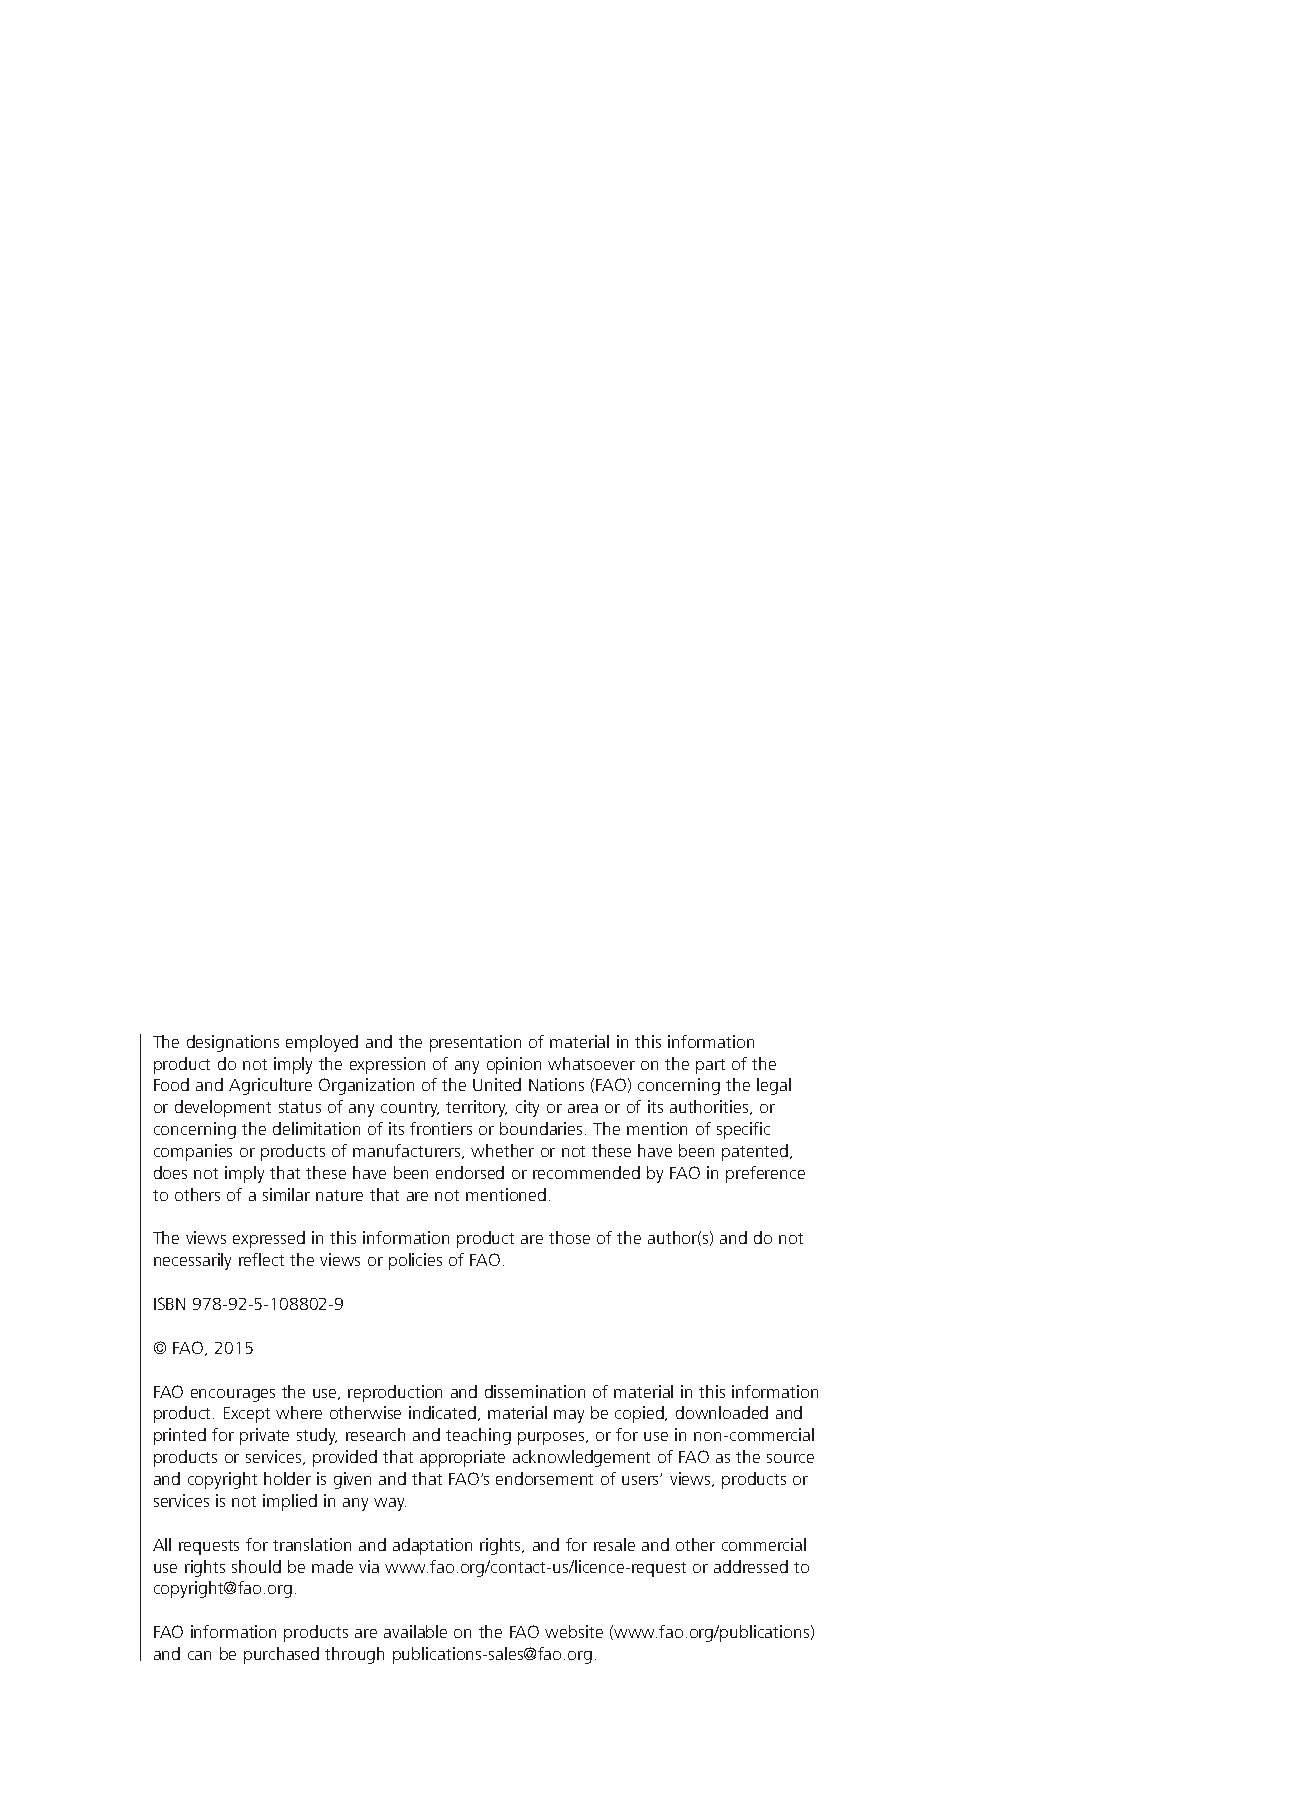
\includepdf[width=\paperwidth,height=\paperheight, offset=-30 -100]{./I4691E_disclaimer.pdf}
\else
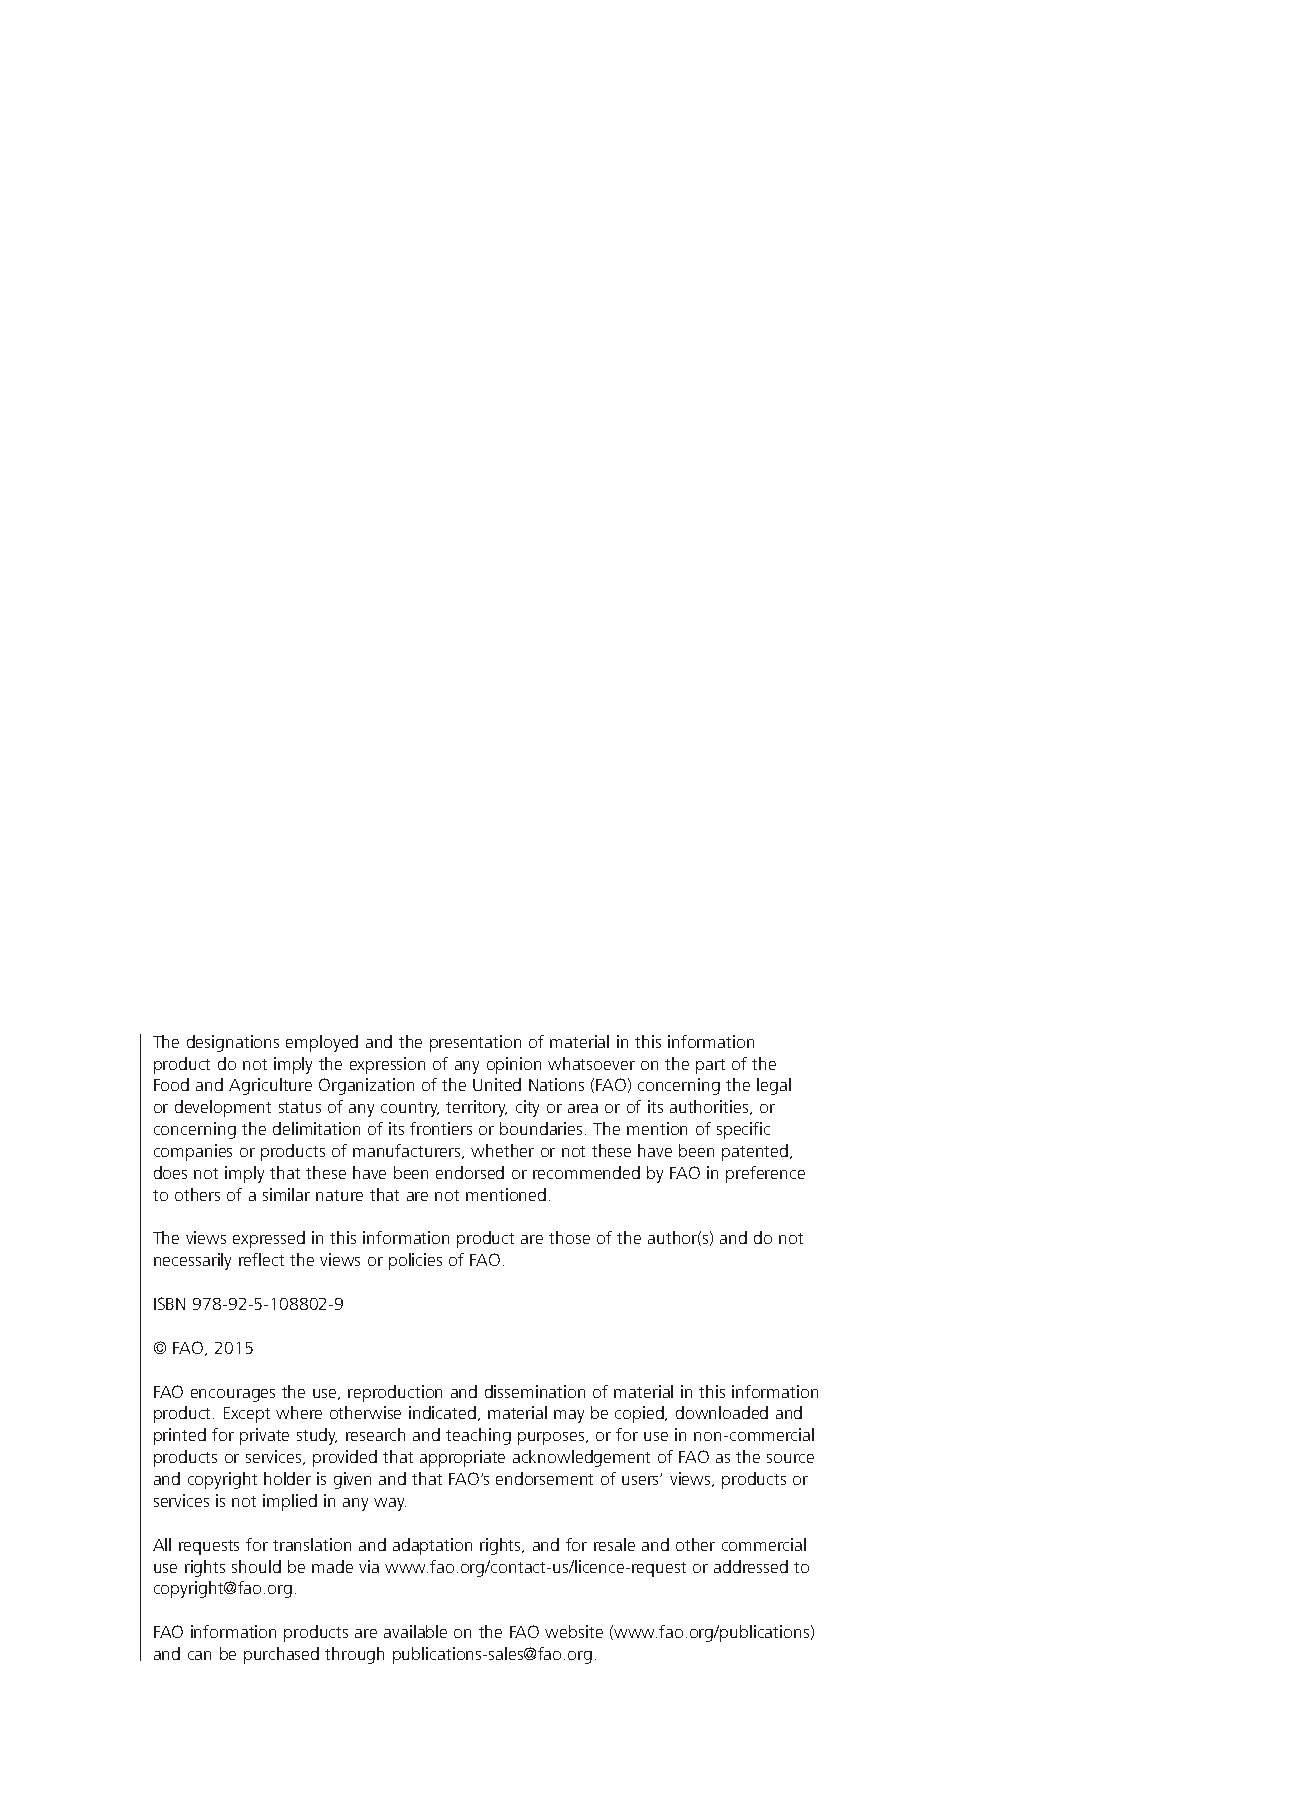
\includepdf[width=\paperwidth,height=\paperheight, offset=-10 -50]{./I4691E_disclaimer.pdf}
\fi


%% List of countries
%\phantomsection
%\renewcommand{\indexname}{List of countries} 
%\addcontentsline{toc}{section}{List of countries}
%\printindex

%%% List of tables
%\phantomsection
%\addcontentsline{toc}{section}{List of Tables}
%\listoftables

%% To be commented if we want to show the List of countries
% \thispagestyle{empty}
% \mbox{}
% \clearpage

%% New part - Introduction
\newpart{white}
%\addtocounter{page}{1}
%\cleardoublepage
\pagenumbering{arabic}  %% Arabic page numbering
\setlength{\parskip}{3pt plus 3pt minus 1pt}  %% Increasing the spacing in the introduction page


% ###########################################################################
% #
% #    _(9(9)__        __/^\/^\__
% #   /o o   \/_     __\_\_/\_/_/_
% #   \___,   \/_   _\.'       './_      _/\_
% #   `---`\  \/_ _\/           \/_   _|.'_/
% #             \  \/_\/      /      \/_  |/ /
% #              \  `-'      |        ';_:' /
% #              /|          \      \     .'
% #             /_/   |,___.-`',    /`'---`
% #           /___/`       /____/
% ###########################################################################

\Large{Foreword}

\bigskip
\bigskip
\bigskip

\large

This year, 2015, is a pivotal one as we look back on the progress we have made on the development agenda, and forward on what we must still accomplish. 

This is the end of a 15-year cycle where the international community partnered with developing countries to tackle the Millennium Development Goals. We are now taking stock of what we can learn from that effort. For example we know that the commitment to halve the percentage of hungry people, that is, to reach the MDG 1c target, has been almost met at the global level. Indeed, 72 of the 129 countries monitored for progress have reached that MDG target, while 29 of them also reached the more ambitious WFS goal by at least halving the number of undernourished people in their populations. 

This year also marks the beginning of the new post-2015 Sustainable Development Agenda. Again the international community will unite around new priorities for the future.

Clear indicators to measure progress towards these international goals is of paramount importance. Timely and robust statistics are the fundamental tool in monitoring the myriad efforts being made, both with an eye to early detection of problems and the recognition of success. The better the data, the better the policies that can be designed. And the better the data, the easier it is to measure the impact of policies or to hold stakeholders accountable for the pledges they make. 

This publication presents selected key indicators related to agriculture and food security that stakeholders can use to prioritize their actions. It is divided into two main sections, one thematic and one country-specific. It presents a variety of dimensions of agriculture and food security along four main focus areas:


{\textbf{\color{Part1} The setting}} measures the state of the agricultural resource base by assessing the supply of land, labour, capital and inputs, and examining the pressure on the world food system stemming from demographic and macroeconomic change.

{\textbf{\color{Part2} Hunger dimensions}} gauges the state of food insecurity and malnutrition, and highlights the four dimensions – availability, access, stability and utilization – that determine the scale of hunger and the shape of undernourishment.

{\textbf{\color{Part3} Food supply}} evaluates the past and present productive capacity of world agriculture, together with the role of trade, in meeting the world’s demand for food, feed and other products.

{\textbf{\color{Part4} Environment}} examines the sustainability of agriculture in the context of the pressure it exerts on its ecological surroundings, including the interaction of agriculture with climate change.

This Pocketbook is part of the FAO Statistical Yearbook suite of products and is just one of the tools that can be used as building blocks for monitoring progress and formulating policy. It includes data from FAOSTAT as well as from other partners within the organization and in the international community. 

FAO is deeply committed to helping countries strengthen their statistical systems to improve the timeliness and quality of their data. And it will continue to do so through the SDG process.


\bigskip
\bigskip

\hspace*{\fill}
        Pietro Gennari
\hspace*{\fill}\newline

\hspace*{\fill}
        \textit{Chief Statistician and Director, Statistics Division}
\hspace*{\fill}




% ###########################################################################
% #
% #    _(9(9)__        __/^\/^\__
% #   /o o   \/_     __\_\_/\_/_/_
% #   \___,   \/_   _\.'       './_      _/\_
% #   `---`\  \/_ _\/           \/_   _|.'_/
% #             \  \/_\/      /      \/_  |/ /
% #              \  `-'      |        ';_:' /
% #              /|          \      \     .'
% #             /_/   |,___.-`',    /`'---`
% #           /___/`       /____/
% ###########################################################################

%% Prelims
\tableofcontents
% \clearpage % commented because of the font size issue




% \clearpage


% \thispagestyle{empty}
% \mbox{}

% \newpage

% ###########################################################################
% #
% #    _(9(9)__        __/^\/^\__
% #   /o o   \/_     __\_\_/\_/_/_
% #   \___,   \/_   _\.'       './_      _/\_
% #   `---`\  \/_ _\/           \/_   _|.'_/
% #             \  \/_\/      /      \/_  |/ /
% #              \  `-'      |        ';_:' /
% #              /|          \      \     .'
% #             /_/   |,___.-`',    /`'---`
% #           /___/`       /____/
% ###########################################################################

% \section{Introduction}

% \bigskip
% \bigskip

% Overcoming malnutrition in all of its forms – caloric undernourishment, micronutrient deficiencies and obesity – requires a combination of interventions in different areas that guarantee the availability of and access to healthy diets. Among the key areas, interventions are required in food systems, public health systems and the provision of safe water and sanitation. This pocketbook not only focuses on indicators of food security and nutritional outcomes but also on the determinants that contribute to healthy lives. 

% The pocketbook is structured in two sections: 
% \begin{itemize}
% \item Thematic spreads related to food security and nutrition, including detailed food consumption data collected from national household budget surveys,
% \item Comprehensive country and regional profiles with indicators categorized by anthropometry, nutritional deficiencies, supplementation, dietary energy supplies, preceded by their "setting".
% \end{itemize}

% \textit{The setting} provides demographic indicators as well as health status indicators based on mortality patterns and the provision of safe water and sanitation. 

% \textit{Anthropometry} indicators provide information not only on the prevalence of acute and chronic forms of under-nutrition but also on the prevalence of obesity. Their co-existence is often referred to as the double burden of malnutrition. 

% \textit{Nutritional deficiency} indicators reveal food security issues at the national level based on the adequacy of energy supplies; they also reveal the prevalence of micronutrient deficiencies, often referred to as “hidden hunger”. Combined with anthropometric measurements, they allow for the identification of the triple burden of malnutrition (under-nutrition, obesity and hidden hunger). Regarding hidden hunger, indicators concerning iodine and vitamin A have been selected.

% \textit{Dietary} indicators are based on national food supplies and inform on the overall quality of diets. Focus is also on the importance of diets during the first 1\,000 days of an infant’s life, with indicators selected on the quality of breastfeeding, dietary diversity and meal frequency. 

% The choice of indicators was guided by the following criteria: relevance to health, food security and nutrition, comparability over time, and availability, in particular for low-income countries. But the criteria were relaxed for several indicators given their importance and the lack of available substitutes. It is hoped that the presence of data gaps will bring about greater efforts to collect the necessary information because only with timely and reliable data can interventions be designed and targeted towards those in most need. Wherever available, disaggregated data by gender have been provided. Such data are indeed key to mainstreaming gender in policies and programmes.

% ###########################################################################
% #
% #    _(9(9)__        __/^\/^\__
% #   /o o   \/_     __\_\_/\_/_/_
% #   \___,   \/_   _\.'       './_      _/\_
% #   `---`\  \/_ _\/           \/_   _|.'_/
% #             \  \/_\/      /      \/_  |/ /
% #              \  `-'      |        ';_:' /
% #              /|          \      \     .'
% #             /_/   |,___.-`',    /`'---`
% #           /___/`       /____/
% ###########################################################################



\setlength{\parskip}{0pt}  %% Restoring the normal spacing


\normalsize

\makeatletter\clearpage\ifodd\c@page\hbox{}\newpage\fi\makeatother %% Remove the colored strip from the introduction page


%%%%%%%%%%%%%%%%%%%%%%%%%%%%%%%%%%%%%%%%%%%%%%%%%%
%% Spreads start from here !!!!
%%%%%%%%%%%%%%%%%%%%%%%%%%%%%%%%%%%%%%%%%%%%%%%%%%



%
%                         .^^^\ ../~/\       .==...==.
%                        .^\ /\  \    ^-------^^ O    O,
%                       / \  \/    ---         ,..++---,
%                      / \_\-          _,v.v^V^ ,/\^^^/
%                     | \/       /^v^V^   _,.-^^  .;+^
%                      \-\   (   \..,+-=~^   .-+/^
%                       \--.__________.--+'^^
%                    ...^--.__________.---^^^^~+._
%   _            _,=^\                            ".
%   \'\.       .^           FFFFF                   '
%    \-/\     /  \          F  FF           )   /    \
%     \-/\   | -      /        FF           )^`\,... |
%     /\-\)  | ,,../^^\        FF           /  /     \
%    /\.-\)  |^     \  \       FF          /  (      )
%   /\. \/   (     \/  /\      FF         /    \/_/_/
%  /==)-/\_   \_\_\/ / |      FFFF       )|
% (=== /. /^^^~~~~~^^\  \               ) |
% (/:/:/ /. /  /  /   \  ^+..........,^^  /
%  \/:/:(:.(:.(:.(  (  \,             ,.;|
%   \$$(:(:(::(::(::(::: ^^""""""""""^  /\
%    ^=U$$$$$Sb\;:\;:\:''"*********+++_/ \)
%        ^"=*UUU$$$$$++ /$$$$&&PP!*=/^\ \/
%                   |++|            \+ + \_ _
%                  _/ . \_           \ .  ___>
%               <(^ /  |__)>          `--.___>
%                 \/^\/
%
%% PART1 - The Setting
%%%%%%%%%%%%%%%%%%%%%%%%%%%%%%%%%%%%%%%%%%%%%%%%%%

\newpart{part1}
\rowcolors{1}{part1!10}{white}
\clearpage













